\chapter{Pairs Trading and Cointegration}
\label{ch:pairs_cointegration}
\chaptermark{Pairs trading and cointegration}

Two stocks move together. When the spread widens, short the winner
and buy the loser; when it narrows, close the position and pocket
the difference. That is \emph{pairs trading} in one sentence, and
the strategy is seductive because it is market-neutral by
construction (long one name, short another) and the thesis
(``these two belong together'') is weaker than predicting
direction.

This chapter shows when the strategy works and why
\emph{correlation is not enough}. Screening for high-correlation
pairs and trading the spread is the single most expensive beginner
mistake; the correct test, \textbf{cointegration}, differs from
correlation in a way invisible to the naked eye but routinely
takes whole strategies offline. We develop both concepts, give the
standard econometric machinery (Engle--Granger, Johansen), and
show that once a cointegrated pair is found the trading rule is
the Ornstein--Uhlenbeck $z$-score machinery of
\cref{ch:mean_reversion_ou}: the cointegration residual is an OU
process, and every formula from that chapter transfers unmodified.

\paragraph{Symbol anchors.} $\beta$ --- cointegrating coefficient
(hedge ratio); $\hat\epsilon_t$ --- cointegration residual (spread);
$z_t$ --- spread $z$-score; $h_{1/2}$ --- half-life; $\theta$ ---
mean-reversion speed.

\begin{backgroundbox}[Prerequisites]
From earlier in the book:
\begin{itemize}
  \item \Cref{ch:mean_reversion_ou}: the OU machinery. Closed-form
  solution, stationary standard deviation
  $\sigma_\infty = \volat/\sqrt{2\theta}$, half-life
  $h_{1/2} = (\ln 2)/\theta$, AR(1) discrete-time mapping,
  augmented Dickey--Fuller (ADF) stationarity test, $z$-score
  entry/exit rule. All of it carries over.
  \item \Cref{ch:spreads_roll}: the Roll model --- first appearance
  of a stationary linear combination (successive trade-price
  differences) inside a non-stationary process (trade prices).
  Cointegration is the multivariate generalisation.
  \item \Cref{ch:price_value}: wall-mid is the reference price for
  any Prosperity spread, since marketable orders execute against
  the far side of the wall.
  \item Forward reference: \cref{ch:backtesting} for walk-forward
  discipline that prevents look-ahead bias when the cointegration
  coefficient is refit in time.
\end{itemize}
From outside the book:
\begin{itemize}
  \item OLS regression $y_t = \alpha + \beta z_t + \epsilon_t$, and
  the fact that swapping $y$ and $z$ produces a different slope.
  \item Random walks: $X_t = X_{t-1} + \eta_t$ with iid $\eta_t$,
  $\Var[X_t - X_0] = t\sigma_\eta^2$. Every individual price in
  this chapter is a random walk; the magic is in linear
  combinations.
\end{itemize}
\end{backgroundbox}

\section{Correlation vs cointegration: the canonical counter-example}
\label{sec:ch10_corrvscoint}

In casual use, ``correlated'' is a synonym for ``related''; in
pairs trading the technical meaning is narrower and misleading if
treated as a substitute for the right test, which is
\emph{cointegration}. The two concepts do not measure the same
thing.

\begin{definition}[Sample correlation of returns]
\index{correlation!sample returns|textbf}
\label{def:return_corr}
For two time series $Y_t$, $Z_t$ sampled at uniform intervals,
the \emph{return correlation} is the Pearson correlation of the
one-period changes,
\begin{equation}
  \Corr(\Delta Y,\,\Delta Z)
  \;=\; \frac{\Cov(\Delta Y_t,\,\Delta Z_t)}
              {\sqrt{\Var[\Delta Y_t]\,\Var[\Delta Z_t]}},
  \qquad \Delta Y_t \defeq Y_t - Y_{t-1}.
\end{equation}
This is a \emph{short-horizon} same-direction-of-motion measure:
``when one goes up, does the other go up at the same instant?''
\end{definition}

\begin{definition}[Cointegration of two series]
\index{cointegration|textbf}
\label{def:cointegration}
Two time series $Y_t$, $Z_t$ are \emph{cointegrated} if there
exists a constant $\beta \in \R$ such that the linear combination
$Y_t - \beta Z_t$ is \emph{stationary}, even though $Y_t$ and
$Z_t$ themselves are non-stationary (typically random walks). The
constant $\beta$ is the \emph{cointegration coefficient} or
\emph{hedge ratio}. The stationary combination
$\hat\epsilon_t \defeq Y_t - \beta Z_t$ is the
\emph{cointegration residual} or \emph{spread}.
\end{definition}

The definitions live on different time horizons. Return correlation
asks about \emph{steps} (changes from one observation to the next);
cointegration asks about \emph{levels} (the long-run tendency of a
linear combination to stay near a constant). A pair can have either
property without the other. Plain-English version: two stocks can be
highly correlated --- both rise in a bull market, both fall in a
crash --- without being cointegrated. Cointegration is the stronger
claim that their \emph{spread} is stationary: any deviation from the
long-run level is temporary and mean-reverts. Correlation is about
co-movement; cointegration is about a tether. Two examples drive the
point home.

\subsection{Counter-example 1: spurious correlation of two random walks}
\label{subsec:ch10_yule}

Take two independent Gaussian random walks starting at the same
point,
\begin{equation}
  Y_t \;=\; Y_{t-1} \;+\; \eta^Y_t,
  \qquad
  Z_t \;=\; Z_{t-1} \;+\; \eta^Z_t,
  \qquad
  Y_0 = Z_0 = 100,
  \label{eq:two_indep_rw}
\end{equation}
with $\eta^Y_t, \eta^Z_t \overset{\iid}{\sim} \Normal(0, 1)$
independent. The two series share no common noise, so the
population return correlation is zero.

But the sample correlation of the \emph{levels} $Y_t, Z_t$ over a
finite window is nearly uniform on $[-1, +1]$. This is Yule's
(1926) \emph{spurious correlation}: any two random walks drift, and
over a finite window those drifts line up by accident.

\paragraph{Numerical demonstration.} Simulate $20$ independent pairs
of $1000$-step Gaussian random walks (different seeds; both starting
at $100$; iid $\Normal(0, 1)$ innovations). Across $20$ seeds the
return correlation stays in $[-0.04,\, +0.08]$ around zero, but the
level correlation ranges from $-0.80$ to $+0.88$, typical absolute
value above $0.4$. A credulous screen would flag these independent
walks as ``strongly correlated.'' Trading the spread $Y_t - Z_t$
is throwing money away: the spread is itself a random walk
(variance doubled) with no tendency to revert.

\begin{historybox}
Yule's ``Why do we sometimes get nonsense-correlations between
time series?'' (1926) is the first formal warning. Granger and
Newbold (1974, ``Spurious regressions in econometrics'')
sharpened the point: $t$-statistics from a regression of one
random walk on another are misleadingly large, and naive
hypothesis tests reject the (true) null far more often than
nominal size suggests. The 1980s cointegration literature grew
out of fixing this.
\end{historybox}

\subsection{Counter-example 2: cointegration without obvious return correlation}
\label{subsec:ch10_cointexample}

Now flip it around. Construct
\begin{equation}
  Y_t \;=\; Y_{t-1} \;+\; \eta_t,
  \qquad
  Z_t \;=\; Y_t \;+\; e_t,
  \label{eq:cointegrated_pair}
\end{equation}
where $\eta_t \overset{\iid}{\sim} \Normal(0,\,1)$ is $Y$'s random
walk innovation, and $e_t$ is an independent
\emph{Ornstein--Uhlenbeck process} with mean $0$, mean-reversion
speed $\theta = 0.3$, and instantaneous volatility $\volat_e = 1$.
$Y_t$ is a random walk; $Z_t$ is the same random walk plus a small
mean-reverting overlay. The spread $Y_t - Z_t = -e_t$ is OU, hence
stationary by construction.

Return correlation is high but not unity:
$\Delta Y_t = \eta_t$, $\Delta Z_t = \eta_t + (e_t - e_{t-1})$, so
they share $\eta_t$ but $\Delta Z_t$ also picks up the OU
innovation. A $5000$-step simulation gives return correlation
$\approx 0.74$ and level correlation $\approx 0.999$. The spread
has stationary variance $\volat_e^2/(2\theta) = 1/0.6 \approx 1.67$,
and ADF rejects the random-walk null with $t \approx -26$ and
$p$-value $\approx 0$. The pair is cointegrated; trading the
spread as an OU process makes money in expectation.

Contrast with \cref{subsec:ch10_yule}: independent random walks
can exhibit level correlation $+0.85$ by accident, while the
constructed cointegrated pair has return correlation $0.74$ from a
genuinely shared walk. \emph{Neither correlation number tells you
which case you are in.} The only distinguishing test takes the
residual of the linear combination and ADF-tests it for
stationarity.

\subsection{The 2x2 table}
\label{subsec:ch10_2x2}

The four combinations of (high/low return correlation) $\times$
(cointegrated/not) are below. Top-left is the target; top-right is
the trap naive screens fall into; bottom-left is the unusual
counter-example we just constructed; bottom-right is the default.

\begin{center}
\renewcommand{\arraystretch}{1.4}
\begin{tabular}{p{3.4cm} p{4.6cm} p{4.6cm}}
\toprule
                           & \textbf{Cointegrated}
                           & \textbf{Not cointegrated} \\
\midrule
\textbf{High return correlation}
  & Move together \emph{and} revert to each other. The pairs
    trader's target. Spread has a half-life $\sim$ days.
  & Move together but drift apart over time. The spread
    diverges. Looks like a pair, is not. \emph{The trap.} \\
\textbf{Low return correlation}
  & Steps look unrelated, but a particular linear combination is
    pinned. Less common; arises e.g.\ when the OU overlay
    dominates the shared random walk on a per-step basis.
  & Independent series. No pair to trade. The default
    case for unrelated names. \\
\bottomrule
\end{tabular}
\end{center}

``Move together and drift apart'' (top right) is what happens to
two trending stocks in the same sector riding the market upward:
daily returns highly correlated (same beta), levels diverge
(idiosyncratic drift). Selling the spread on a correlation screen
leaves you short the winner and long the loser for as long as the
trend continues --- months.

\begin{pitfallbox}[Don't pairs-trade on correlation alone]
Any two well-known equities --- two gold miners, two US banks,
two oil majors --- can show return correlation above $0.9$ over
a multi-year sample (same factor exposure). Yet the spread can
drift to infinity if earnings or operating leverage diverge. A
trader who screens for ``correlation $> 0.9$'', sells the high one
and buys the low one is \emph{trend-fighting}, not mean-reverting
--- the spread has no level to revert to. The right test: regress,
take the residual, ADF-test it; only if ADF rejects is the pair
tradeable. \citeChan{} (Chapter 2) is the practitioner reference.
\end{pitfallbox}

\section{The Engle--Granger two-step}
\label{sec:ch10_engle_granger}

Engle and Granger (1987) proposed the \emph{Engle--Granger two-step}
test for cointegration. Five lines of Python, and it remains the
standard first-pass test on a stat-arb desk.

\subsection{Step 1: estimate the hedge ratio by OLS}
\label{subsec:ch10_eg_step1}

Run OLS of $Y_t$ on $Z_t$ with an intercept,
\begin{equation}
  Y_t \;=\; \alpha \;+\; \beta\,Z_t \;+\; \epsilon_t,
  \label{eq:eg_regression}
\end{equation}
where $(\alpha, \beta)$ minimise the sum of squared residuals over
the fitting window. OLS returns
\begin{equation}
  \hat\beta \;=\; \frac{\Cov(Y_t,\,Z_t)}{\Var(Z_t)},
  \qquad
  \hat\alpha \;=\; \bar{Y} - \hat\beta\,\bar{Z},
  \label{eq:eg_ols_formulae}
\end{equation}
where bars denote sample means over the fitting window.

The slope $\hat\beta$ is the \emph{cointegration coefficient} or
\emph{hedge ratio}: the units of $Z$ to short per unit of $Y$ long
to make the spread $Y - \beta Z$ as quiet as possible. The
intercept $\hat\alpha$ absorbs the average level difference.

\subsection{Step 2: test the residual for stationarity}
\label{subsec:ch10_eg_step2}

Compute the residual
\begin{equation}
  \hat\epsilon_t \;\defeq\; Y_t - \hat\alpha - \hat\beta\,Z_t,
  \label{eq:eg_residual}
\end{equation}
and run an ADF test (\cref{ch:mean_reversion_ou}) on
$\hat\epsilon_t$. The logic: $Y_t$ and $Z_t$ are each random walks
(non-stationary), so OLS can \emph{always} find coefficients that fit
them against each other; the question is whether the leftover
residual $\hat\epsilon_t$ is itself stationary (pair is cointegrated,
spread is tradeable) or another random walk (regression was
spurious, pair is not cointegrated). One wrinkle: because $\hat\beta$ was estimated,
the standard ADF critical values are wrong. Corrected values
tabulated by Engle--Granger (1987) and updated by MacKinnon
(1991) are modestly more demanding; the corrected test is the
\emph{Engle--Granger CADF}. Every package implements both; call
the right one.

If (C)ADF rejects the random-walk null, a stationary linear
combination exists --- the pair is cointegrated. Failure to reject
(given ADF's low power) is inconclusive; the prudent action is not
to trade the pair.

\begin{keyfactbox}[Engle--Granger two-step]
Given two candidate price series $\{Y_t\}$, $\{Z_t\}$ over a
fitting window:
\begin{enumerate}
  \item Run OLS on \eqref{eq:eg_regression}: $Y_t = \alpha
  + \beta Z_t + \epsilon_t$. Read off
  $(\hat\alpha,\,\hat\beta)$ from \eqref{eq:eg_ols_formulae}.
  \item Compute residuals
  $\hat\epsilon_t = Y_t - \hat\alpha - \hat\beta Z_t$.
  \item Run an ADF test (with cointegration-corrected critical
  values) on $\hat\epsilon_t$. Reject the random-walk null at
  $5\%$ $\Rightarrow$ the pair is cointegrated.
  \item If cointegrated, the hedge ratio is $\hat\beta$ and
  the spread is $\hat\epsilon_t$. Treat $\hat\epsilon_t$ as an
  OU process and apply the
  \cref{ch:mean_reversion_ou} machinery.
\end{enumerate}
\end{keyfactbox}

\subsection{Worked example: EWA / EWC}
\label{subsec:ch10_ewa_ewc}

The canonical practitioner pair is \textbf{EWA} (iShares MSCI
Australia) and \textbf{EWC} (iShares MSCI Canada). These ETFs
(exchange-traded funds: securities holding a basket of stocks and
trading like a single share; formal definition in
\cref{ch:basket_etf_arb}) track two commodity-exporter economies
with similar industrial composition (mining, energy, banks), so
they move together. Chan (\citeChan{}, Chapter 2) runs the
cointegration analysis on early-2000s daily data:
\begin{itemize}
  \item OLS hedge ratio $\hat\beta \approx 0.75$ (EWA on EWC): one
  unit long EWA hedges with $0.75$ units short EWC.
  \item CADF $t \approx -3.7$, $p \approx 0.005$ --- cointegrated.
  \item Residual half-life $\approx 7$ trading days.
  \item $\sigma_\infty$ a few percent of spot ETF price.
\end{itemize}
Plug these into the OU machinery from
\cref{ch:mean_reversion_ou}. The half-life is
$h_{1/2} \approx 7$ days, so $\theta = (\ln 2)/7 \approx 0.099$
per day. With entry threshold $z_{\text{entry}} = 2$ and exit
threshold $z_{\text{exit}} = 0.5$ the expected duration of a
single trade is, by \eqref{eq:zscore_duration} of
\cref{ch:mean_reversion_ou},
\begin{equation}
  h \;=\; \frac{1}{\theta}\,\ln\!\left(\frac{2}{0.5}\right)
       \;=\; \frac{\ln 4}{0.099}
       \;\approx\; 14 \text{ trading days},
  \label{eq:ewa_ewc_duration}
\end{equation}
i.e.\ a typical EWA/EWC round trip lasts a couple of weeks. With
a couple of trades per quarter and target reversion of three to
four residual standard deviations, historical Sharpe is
$1$--$1.5$ (Chan) --- modest, consistent, and uncorrelated with
market direction. Modern alpha on this exact pair has decayed
(\cref{sec:ch10_failure_modes}), but the geometry is the canonical
teaching example.

\begin{pitfallbox}[The cointegration vector is not symmetric]
\label{pitfall:asymmetric}
Which series goes on the left ($Y_t$, dependent) vs right ($Z_t$,
regressor) matters. OLS minimises squared residuals along the $Y$
axis only, so swapping changes the slope. Regressing EWA on EWC
might give $\hat\beta_{Y\mid Z} \approx 0.75$, EWC on EWA
$\hat\beta_{Z\mid Y} \approx 1.10$ ($1/0.75 = 1.33$, so
$\hat\beta_{Y\mid Z}\cdot\hat\beta_{Z\mid Y} \neq 1$ unless the
regression is noiseless --- the regression-to-the-mean fallacy).
The two regressions produce different residuals and, near the $5\%$
threshold, different test outcomes.

Fix, in order of preference: (i) put the higher-variance series on
the right; (ii) use total least squares (orthogonal regression);
(iii) use Johansen (\cref{sec:ch10_johansen}), invariant to
ordering. Chan (\citeChan{}, Chapter 2) recommends running both
directions; if they disagree, the pair is not robustly cointegrated.
\end{pitfallbox}

\section{The Johansen test (stated)}
\label{sec:ch10_johansen}

For two assets, Engle--Granger is adequate. For three or more,
two problems appear: (i) the choice of left-hand-side asset
becomes a combinatorial mess; (ii) a basket of $n$ assets can have
\emph{multiple} cointegration relationships (up to $n-1$), but
Engle--Granger finds at most one. The \textbf{Johansen test}
(Johansen, 1988, 1991) solves both in vector form.

The setting is a vector \emph{error-correction model} (VECM) for an
$n$-dimensional process $\bm X_t = (X_{1,t}, \ldots, X_{n,t})^\top$,
\begin{equation}
  \Delta \bm X_t \;=\; \Pi\,\bm X_{t-1}
                       \;+\; \sum_{i=1}^{p-1}\Gamma_i\,\Delta\bm X_{t-i}
                       \;+\; \bm\mu \;+\; \bm\epsilon_t,
  \label{eq:vecm}
\end{equation}
with $\Pi$, $\Gamma_i$ as $n\times n$ matrices, $\bm\mu$ an
intercept, $\bm\epsilon_t$ multivariate noise. The matrix $\Pi$
is the long-run impact. Three cases for its rank
$r \defeq \operatorname{rank}\Pi$:
\begin{itemize}
  \item $r = 0$: $\Pi = 0$, the VECM collapses to a pure VAR in
  differences, no stationary linear combination exists, no
  cointegration.
  \item $r = n$: $\Pi$ is full rank, $\bm X_t$ is stationary, no
  random-walk component.
  \item $0 < r < n$: exactly $r$ independent stationary linear
  combinations. $\Pi$ factors as $\Pi = \alpha \beta^\top$ where
  $\alpha, \beta$ are $n \times r$; columns of $\beta$ are the
  \emph{cointegration vectors} (each a stationary combination of
  $\bm X_t$), and $\alpha$ is the \emph{adjustment matrix} (how
  strongly each component pulls back toward the stationary level).
\end{itemize}
Johansen estimates $r$ via likelihood-ratio tests on the
eigenvalues of $\Pi$. Two statistics: \emph{trace} tests
$H_0: r \leq r_0$ for $r_0 = 0, \ldots, n-1$;
\emph{maximum-eigenvalue} tests $H_0: r = r_0$ against
$H_1: r = r_0 + 1$. Both have non-standard distributions tabulated
by Johansen. Derivation omitted; \citeHasbrouck{} treats the
vector-cointegration setting, and \citeCartea{} (Chapter 13) gives
an algorithmic treatment.

The pipeline is one library call:
\texttt{statsmodels.tsa.vector\_ar.vecm.coint\_johansen} takes a
$T\times n$ price matrix and returns trace statistic,
max-eigenvalue statistic, and estimated cointegration vectors.
Read the rank by comparing each statistic to its critical value;
the columns of the cointegration matrix are the basket weights.

\begin{intuitionbox}
Johansen finds every stationary linear combination at once. For
two assets, it matches Engle--Granger. For $n$ assets, it reports
how many \emph{independent} stationary combinations exist: five
sector stocks might yield three mispricing factors to trade, or
zero. Engle--Granger cannot discover this multi-relationship
structure because it bakes in a single left-hand-side regression.
\end{intuitionbox}

\section{Trading the residual as an OU process}
\label{sec:ch10_trading}

Once a test has produced $\hat\beta$ and residuals
$\hat\epsilon_t$, the trading rule is the $z$-score OU strategy
from \cref{ch:mean_reversion_ou} applied to $\hat\epsilon_t$ ---
every formula transfers unmodified.

\subsection{Recap of the OU machinery on the residual}
\label{subsec:ch10_recap_ou}

Treat $\hat\epsilon_t$ as OU. By the AR(1) mapping of
\cref{ch:mean_reversion_ou} (equation
\eqref{eq:ou_ar1_reparam}), regressing $\hat\epsilon_{t+1}$ on
$\hat\epsilon_t$ recovers
$(\hat\theta_\epsilon,\, \hat\mu_\epsilon,\, \hat\volat_\epsilon)$.
Then $h_{1/2} = (\ln 2)/\hat\theta_\epsilon$,
$\hat\sigma_\infty = \hat\volat_\epsilon/\sqrt{2\hat\theta_\epsilon}$,
and the live $z$-score
\begin{equation}
  z_t \;\defeq\; \frac{\hat\epsilon_t - \hat\mu_\epsilon}
                      {\hat\sigma_\infty}.
  \label{eq:residual_z}
\end{equation}
Apply the entry / exit / stop-out rule of
\cref{ch:mean_reversion_ou}: enter when $|z_t| > z_{\text{entry}}$,
exit when $|z_t| < z_{\text{exit}}$, stop out when
$|z_t| > z_{\text{stop}}$. Expected trade duration is
$h \approx \theta_\epsilon^{-1}\ln(z_{\text{entry}}/z_{\text{exit}})$.

\begin{figure}[ht]
\centering
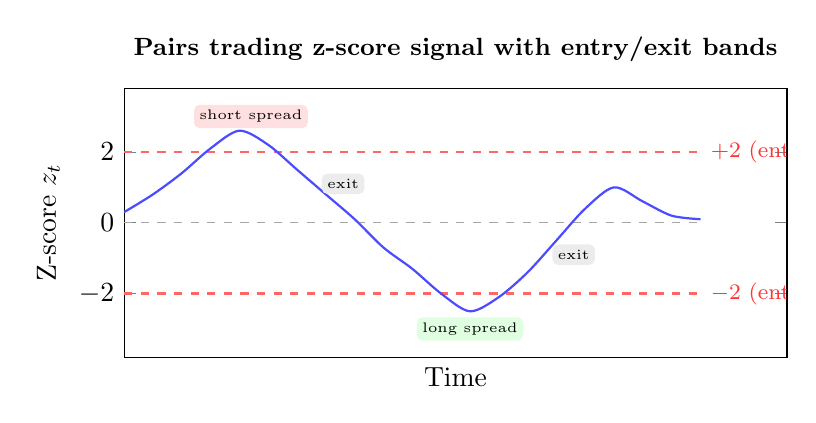
\begin{tikzpicture}
\begin{axis}[
  width=10cm, height=5cm,
  xlabel={Time},
  ylabel={Z-score $z_t$},
  xmin=0, xmax=10,
  ymin=-3.8, ymax=3.8,
  ytick={-2,0,2},
  xtick=\empty,
  grid=none,
  enlarge x limits={upper,value=0.15},
  title={Pairs trading z-score signal with entry/exit bands},
  title style={font=\small\bfseries},
]
\addplot[dashed, black!35, thin] coordinates {(0,0)(10,0)};
\addplot[dashed, red!60, thick]
  coordinates {(0,2)(10,2)}
  node[right, font=\footnotesize, red!80]{$+2$ (entry short)};
\addplot[dashed, red!60, thick]
  coordinates {(0,-2)(10,-2)}
  node[right, font=\footnotesize, red!80]{$-2$ (entry long)};
\addplot[blue!70, thick, smooth] coordinates {
  (0,0.3)(0.5,0.8)(1.0,1.4)(1.5,2.1)(2.0,2.6)(2.5,2.2)(3.0,1.5)
  (3.5,0.8)(4.0,0.1)(4.5,-0.7)(5.0,-1.3)(5.5,-2.0)(6.0,-2.5)
  (6.5,-2.1)(7.0,-1.4)(7.5,-0.5)(8.0,0.4)(8.5,1.0)(9.0,0.6)(9.5,0.2)(10,0.1)
};
\node[fill=red!12, rounded corners=2pt, font=\tiny, inner sep=2pt]
  at (axis cs:2.2, 3.0) {short spread};
\node[fill=gray!15, rounded corners=2pt, font=\tiny, inner sep=2pt]
  at (axis cs:3.8, 1.1) {exit};
\node[fill=green!12, rounded corners=2pt, font=\tiny, inner sep=2pt]
  at (axis cs:6.0,-3.0) {long spread};
\node[fill=gray!15, rounded corners=2pt, font=\tiny, inner sep=2pt]
  at (axis cs:7.8,-0.9) {exit};
\end{axis}
\end{tikzpicture}
\caption{Pairs-trading z-score signal. The strategy shorts the spread when
$z_t > +2$ (spread too wide relative to history) and goes long when
$z_t < -2$ (spread too narrow). Both positions are closed when $z_t$
reverts to zero. The $\pm 2$ thresholds are chosen to balance
entry frequency against the probability of a false signal.}
\label{fig:zscore_bands}
\end{figure}

\subsection{What ``a position'' means in a pair trade}
\label{subsec:ch10_position}

The trade is on the spread, not on either name:
\begin{itemize}
  \item \textbf{Long the spread} ($z_t < -z_{\text{entry}}$,
  residual too low): buy $1$ unit of $Y$, sell $\hat\beta$ units
  of $Z$. Zero net dollar exposure to a parallel rally.
  \item \textbf{Short the spread} ($z_t > +z_{\text{entry}}$,
  residual too high): sell $1$ unit of $Y$, buy $\hat\beta$ units
  of $Z$.
\end{itemize}
$\hat\beta$ is the literal short-leg sizing. At
$\hat\beta = 0.75$ (EWA/EWC), every $\$100$ long EWA pairs with
$\$75$ short EWC: notional $\$175$, net-market exposure $\$25$.

\subsection{Refitting the hedge ratio: how often?}
\label{subsec:ch10_refit}

$\hat\beta$ is not fixed. Like the OU parameters, it drifts as
businesses evolve: a mining company shifts asset mix, an ETF
rebalances, a rate-regime change shifts two banks' sensitivities.
The fix is walk-forward fitting from \cref{sec:ch9_walkforward}:
pick a fitting window $W$ and refit cadence $R$, recompute
$\hat\beta$ on the most recent $W$ observations using only data
strictly before each refit timestamp.

$W$ and $R$ trade off. Long $W$ gives stable $\hat\beta$ but
adapts slowly. Short $W$ adapts fast but produces noisy slopes.
Short $R$ refits often but turns $\hat\beta$ into an overfittable
parameter. Rules of thumb (Chan, \citeChan{} Chapter 3) for
daily equity pairs: $W = 250$ days, $R = 21$ (monthly), or
$W = 90$, $R = 5$ for faster signals. For Prosperity tick data,
scale both by ticks-per-round.

\begin{pitfallbox}[Don't over-refit \texorpdfstring{$\hat\beta$}{the hedge ratio}]
Refitting $\hat\beta$ every bar introduces look-ahead and
overfitting two ways.

First, if refit at $t$ uses $[t - W,\, t]$ (\emph{including}
$Y_t, Z_t$), then $\hat\beta_t$ depends on the current
observation, and $\hat\epsilon_t = Y_t - \hat\alpha_t -
\hat\beta_t Z_t$ is mechanically biased toward zero. The strategy
then buys low and sells high against a mean that already knows the
current realisation. Backtests look spectacular; live is noise.

Second, even using only data strictly before $t$, a one-bar refit
cadence wastes degrees of freedom: each fit yields a different
hedge ratio, the spread fragments into short stationary pieces,
and OU parameter estimates on each are noisier than on the full
window.

Fix: refit weekly or monthly, hold $\hat\beta$ constant out of
sample until the next refit. Only the $z$-score moves bar by bar.
\end{pitfallbox}

\begin{keyfactbox}[Cointegration + OU is one algorithm]
Pairs trading and OU mean reversion (\cref{ch:mean_reversion_ou})
are the same algorithm with different inputs. The $z$-score code
from \cref{sec:ch9_code} wraps unchanged around a cointegration
residual; the only addition is an upstream Engle--Granger (or
Johansen) fit producing $\hat\beta$ and the residual. Every
downstream formula --- half-life, $\sigma_\infty$, $z$-thresholds,
expected duration, walk-forward refit --- transfers unmodified.
\end{keyfactbox}

\section{A short reference implementation}
\label{sec:ch10_code}

The Engle--Granger pipeline fits in one pure function: two
equal-length numpy arrays in; OLS hedge ratio, intercept, residual
mean, residual standard deviation, and ADF $p$-value out. The OU
machinery is \texttt{fit\_ou} from \cref{sec:ch9_code} applied to
the residual.

\begin{lstlisting}[caption={Engle--Granger two-step as a pure function.}]
import numpy as np
from statsmodels.tsa.stattools import adfuller

def engle_granger(y: np.ndarray, z: np.ndarray) -> dict:
    """Engle-Granger two-step. Returns hedge ratio, residual stats, ADF p-value."""
    # Step 1: OLS regression  y = alpha + beta * z + eps
    beta, alpha = np.polyfit(z, y, 1)
    resid = y - (alpha + beta * z)
    # Step 2: ADF test on the residual
    adf_p = adfuller(resid, autolag='AIC')[1]
    return {
        'alpha': float(alpha),
        'beta':  float(beta),
        'mean':  float(resid.mean()),
        'std':   float(resid.std(ddof=1)),
        'adf_p': float(adf_p),
    }
\end{lstlisting}

Three production notes. First, \texttt{adfuller} returns the
univariate ADF $p$-value, not the CADF-corrected value; for
production use \texttt{statsmodels.tsa.stattools.coint}. Second,
the skeleton silently assumes $\hat\beta > 0$; $\hat\beta \leq 0$
signals a broken regression (can occur for a long ETF and its
inverse, but rare). Third, call this inside a walk-forward loop.
One call on the entire history with cached residual is the
look-ahead trap above.

\begin{prosperitybox}[title={Prosperity example: PICNIC\_BASKET as a cointegration trade}]
The cleanest Prosperity cointegration setup is the \textbf{picnic
basket}: PICNIC\_BASKET contains a fixed multiple of three
underlying products (Prosperity 3: six CROISSANTS, three JAMS,
one DJEMBE). It trades against a ``synthetic basket'' replicated
from constituents. Define
\begin{equation}
  \text{spread}_t \;\defeq\; P_t^{\text{basket}}
  \;-\; \bigl(6\,P_t^{\text{cr}} \;+\; 3\,P_t^{\text{jam}} \;+\; 1\,P_t^{\text{dj}}\bigr).
  \label{eq:basket_spread}
\end{equation}
Each underlying is a random walk; the spread is stationary (mean
reflects basket miscalibration, volatility reflects quote noise).
The hedge ratio is \emph{known}: $\bm\beta = (1, -6, -3, -1)$, no
fitting needed. Engle--Granger is overkill, but OU on the residual
is essential. \Cref{ch:basket_etf_arb} treats the full strategy;
Frankfurt Hedgehogs' Prosperity 3 writeup
(\texttt{imc-prosperity-3/README.md}) trades it on a $z$-score rule.

\textbf{Numerical sanity check.} Frankfurt reported stationary
standard deviation $\approx 40$ seashells and half-life
$\approx 50$ Prosperity timesteps. Plugging $h_{1/2} = 50$ into
$\theta = (\ln 2)/h_{1/2}$ gives $\theta \approx 0.01386$. With
$z_{\text{entry}} = 1.5$, $z_{\text{exit}} = 0.3$, expected
round-trip duration, by \eqref{eq:zscore_duration} of
\cref{ch:mean_reversion_ou}, is
\begin{equation}
  h \;=\; \frac{\ln(1.5/0.3)}{\theta}
       \;=\; \frac{\ln 5}{0.01386}
       \;\approx\; \frac{1.6094}{0.01386}
       \;\approx\; 116 \text{ timesteps}.
  \label{eq:basket_duration}
\end{equation}
More than twice the half-life ($z = 1.5 \to 0.3$ is a factor-$5$
shrink, more than two halvings). Over a $10\,000$-timestep round
expect $80$--$100$ round-trip basket trades on this signal alone,
consistent with Frankfurt's reported counts.
\end{prosperitybox}

\begin{gsbox}
On a cash-equities pairs desk at Goldman (or any sell-side
stat-arb shop), Engle--Granger and Johansen run as a daily
\emph{sweep} over every plausible pair/triple in a sector
universe. Morning workflow:
\begin{enumerate}
  \item \textbf{Universe screen.} One sector at a time (US banks,
  European energy majors, gold miners) --- cross-sector
  cointegration is rare and usually spurious.
  \item \textbf{Johansen sweep.} Johansen on every pair (sometimes
  triple) in the sector basket, rolling $250$--$500$ day window.
  Record trace statistic, rank, cointegration vectors.
  \item \textbf{Half-life filter.} Reject residual half-lives
  shorter than a few days (costs eat the edge) or longer than a
  few weeks (capital tied up). Sweet spot: $3$--$20$ days.
  \item \textbf{Cost gate.} Stationary spread SD must be a few
  multiples of round-trip cost on both legs. A spread reverting
  by $20$ bps is not tradeable if round-trip costs $15$ bps.
  \item \textbf{Sizing.} Convert live $z$-scores into
  Kelly-fraction positions (\cref{ch:kelly_risk}), cap at per-pair
  VaR, feed to the execution algo (\cref{ch:almgren_chriss}).
\end{enumerate}
Division of labour: the \emph{Strat} owns sweep code, the
Engle--Granger/Johansen library, the half-life filter, and Kelly
sizing. The \emph{trader} owns exit-on-fundamentals: an M\&A,
index reweighting, or major analyst downgrade flags a pair as
``cointegration broken'' and the trader pulls the position
regardless of $z$-score. Strats handle statistics and sizing;
traders handle structural breaks the model cannot see.
\end{gsbox}

\section{Failure modes and when pairs trading dies}
\label{sec:ch10_failure_modes}

Pairs trading is not free money. The failure modes, in order of
how often they bite, plus LTCM as the canonical reminder:

\paragraph{Structural breaks in $\hat\beta$.} A merger, index
inclusion or exclusion, regulatory change, or analyst event can
shift the $Y$--$Z$ relationship discontinuously. $\hat\beta$ jumps,
the historical residual stops being stationary at the old level,
and the spread trends to a new equilibrium the model cannot see.
Walk-forward refit catches this only after a loss equal to the
gap between old and new equilibrium. Discipline: hard stop-out on
$|z| > z_{\text{stop}}$, plus a manual ``no-trade'' watchlist for
pairs with imminent earnings, M\&A rumours, or index reweightings.

\paragraph{Transaction costs overwhelm small reversion.} A
half-life of one day with $\sigma_\infty = 20$ bps sounds great
until a US-equity round trip costs $5$--$10$ bps in commissions
and bid-ask, plus the borrow on the short leg. A $z = 2 \to 0.5$
reversion harvests $1.5\sigma_\infty = 30$ bps, more than half of
which goes to costs. The GS cost gate above exists for this.

\paragraph{Convergence timing is unbounded.} The OU model gives
the \emph{expected} reversion time, but the variance is large. A
$3\sigma$ deviation might revert in a day or in six months, and
the position marks to market every step. With leverage --- most
real pairs books use it, since P\&L per unit notional is small ---
a long convergence triggers a margin call before the model says
to give up. Discipline: hard stop-out (\cref{ch:mean_reversion_ou}),
\emph{conservative} Kelly fraction (\cref{ch:kelly_risk}), and
unwind any position that has not reverted within a few half-lives.

\paragraph{Look-ahead through the refit.} Covered in the pitfall
above: a pipeline that fits $\hat\beta$ on data through $t$ to
compute the residual at $t$ is silently cheating and reveals
itself only in live trading.

\paragraph{Decay of historical alpha.} Canonical pairs (EWA/EWC,
Coke/Pepsi, Shell/BP) have had their margins compressed to where
they barely cover costs. Strategies that work in $2005$ papers do
not work in $2026$ on the same pairs at the same parameters. Not
a bug in cointegration --- standard edge erosion. Discipline: keep
finding new candidates, on underexplored sector slices or in
markets with structural barriers to high-frequency entry.

\begin{pitfallbox}[Pair trades are not riskless arbitrage]
\label{pitfall:ltcm}
The cautionary tale is \textbf{Long-Term Capital Management
(LTCM)}, founded 1994 by John Meriwether with Nobel laureates
Scholes and Merton on the board. LTCM ran a vast
cointegration-based portfolio --- on-the-run vs off-the-run
Treasuries, swap spreads across countries, convertible-bond
arbitrage --- with peak notional around $\$1.25$ trillion against
about $\$5$ billion of equity. Their analysis was correct: the
relationships \emph{were} cointegrated and \emph{would} have
reverted given time.

In August 1998 Russia defaulted, investors fled to safety, and
every spread LTCM held widened simultaneously. The relationships
were not broken --- spreads did eventually revert --- but LTCM's
leverage meant marked-to-market losses triggered margin calls
they could not meet. The fund collapsed in September 1998; a
consortium of banks injected $\$3.6$ billion to unwind positions
in orderly fashion. Lowenstein's \emph{When Genius Failed} (2000)
is the canonical narrative.

Lesson: cointegration tells you about the long-run mean.
\emph{It tells you nothing about the worst drawdown along the
way.} The position-sizing rules of \cref{ch:kelly_risk} and the
stop-out rules of \cref{ch:mean_reversion_ou} are the only thing
standing between ``profitable in expectation'' and ``insolvent
before convergence.''
\end{pitfallbox}

\section{Key facts to memorise}
\label{sec:ch10_keyfacts}

\begin{itemize}
  \item \textbf{Correlation $\neq$ cointegration.} Return
  correlation is on \emph{differences}; cointegration is a
  long-run-stationary property of a linear combination of
  \emph{levels}. Only cointegration is the right test for pairs
  trading.
  \item \textbf{Spurious correlation.} Independent random walks
  routinely exhibit sample level correlation across $[-1, +1]$ by
  chance. Screening on level correlation alone throws money away.
  \item \textbf{Engle--Granger two-step.} (1) OLS
  $Y_t = \alpha + \beta Z_t + \epsilon_t$ gives the hedge ratio;
  (2) ADF (with cointegration-corrected critical values) on the
  residual tests stationarity. Reject the random-walk null
  $\Rightarrow$ cointegrated.
  \item \textbf{Asymmetric regression.} OLS in
  \eqref{eq:eg_regression} is not symmetric in $Y$ and $Z$. Fix:
  total least squares, or Johansen.
  \item \textbf{Johansen test.} For $n \geq 2$ assets, estimates
  the rank $r$ of $\Pi$ in a VECM and returns $r$ independent
  cointegration vectors at once. Engle--Granger is the $n=2$ case.
  \item \textbf{Trading rule = OU $z$-score on the residual.} Fit
  $(\hat\theta, \hat\mu, \hat\volat)$ via AR(1) mapping, apply the
  entry/exit/stop rules of \cref{ch:mean_reversion_ou}. No new
  logic.
  \item \textbf{Position sizing.} Long the spread $\Rightarrow$
  buy $1$ unit of $Y$, sell $\hat\beta$ units of $Z$.
  \item \textbf{Walk-forward refit.} Refit $\hat\beta$ on a
  rolling $W$-window every $R$ steps, using only data strictly
  before the refit timestamp. Hold $\hat\beta$ constant out of
  sample. Refitting every bar is the canonical look-ahead trap.
  \item \textbf{Failure modes.} Structural breaks, transaction
  costs, unbounded convergence timing, look-ahead, edge decay.
  \item \textbf{LTCM (1998).} Cointegration correct, convergence
  timing wrong, leverage too high. Risk management is the strategy.
  \item \textbf{Prosperity link.} PICNIC\_BASKET premium is a
  cointegrated spread with known hedge ratio $(1, -6, -3, -1)$;
  \cref{ch:basket_etf_arb} treats it in detail.
  \item \textbf{Goldman link.} Sell-side stat-arb desks run a
  daily Johansen sweep, gate by half-life and cost, size by Kelly;
  trader handles structural-break exits.
\end{itemize}
